\chapter{Zaimplementowane algorytmy}

Zgodnie z założeniami w niniejszej pracy zaimplementowane zostały rozwiązania dla następujących
etapów procesu rozpoznawania tęczówki:

\begin{itemize}
  \item przetwarzanie wstępne,
  \item normalizacja,
  \item kodowanie,
  \item dopasowanie.
\end{itemize}

\noindent
Algorytmy segmentacji tęczówki oraz usuwania zakłóceń zostały pominięte, ponieważ były przedmiotem
innej pracy dyplomowej. W dalszej części rozdziału opisane zostaną zaimplementowane algorytmy
dla wyżej wymienionych etapów.

\section{Przetwarzanie wstępne}

Odpowiednie przygotowanie obrazu przed rozpoczęciem procesu rozpozanawania jest bardzo ważne. Pozwala
ono na polepszenie jakości zdjęcia przez usunięcie zakłóceń czy poprawienie kontrastu, co znacznie
wpływa na jakoś\'c działania całego systemu.\newline

Różne metody segmentacji wymagają odmiennego wstępnego przygotowania obrazu. Często proces przygotowania
obrazu różni się nawet dla poszczególnych etapów procesu segmentacji, tzn. innych operacji może wymaga\'c
obraz w trakcie szukania parametrów źrenicy, a jeszcze innego w trakcie szukania parametrów tęczówki.
Z tego względu przetwarzanie wstępne może byc doś\'c skomplikowane i składac się z wielu różnorodnych
kroków.

Ponieważ algorytmy segmentacji często polegają na konkretnych operacjach przygotowawczych, których może
by\'c wiele, umożliwienie użytkownikowi ich parametryzacji bardzo skomplikowałoby interfejs aplikacji
i znacznie pogorszyło by jego czytelnoś\'c, jednocześnie dając użytkownikowi niewiele pola do manipulacji
tą częścią procesu.\newline

Ze względu na zależnoś\'c procesu przygotowania obrazu od wybranego algorytmu segmentacji, implementacja
przetwarzania wstępnego przeniesiona została do implementacji poszczególnych metod segmentacji,
a użytkownikowi udostępnione zostały wyłącznie uniwersalne algorytmy takie jak:

\begin{itemize}
  \item filtr Gaussa
  \item filtr medianowy
  \item normalizacja histogramu
  \item filter2D
\end{itemize}

Implementacje tych alogrytmów wykorzystują podstawowe funkcje z biblioteki OpenCV takie jak:
\verb|GaussianBlur|, \verb|medianBlur|, \verb|equalizeHist| oraz \verb|filter2D|.

\section{Normalizacja}

Porównywanie tęczówki może by\'c problematyczne, ze względu na potencjalne niezgodności w
wymiarach obrazu. Najczęstszą przyczyną tych niespójności jest zmiana rozmiaru tęczówki
będąca wynikiem rozszerzania lub kurczenia się  \'zrenicy oka w zależności od intensywności
oświetlenia w otoczeniu. Niespójności te mogą wynika\'c również z innych \'zródeł np. różna
odległoś\'c w trakcie pobierania zdjęcia, różnice w obrocie kamery, inna rotacja oka, czy
nawet nachylenie głowy w trakcie pobierania zdjęcia \cite{DaugmanHowIrisRecognitionWorks}.\newline

W celu umożliwienia porównania dwóch obrazów, z których każde mogło by\'c zrobione w odmiennych
warunkach, obraz poddaje się procesowi normalizacji, który ma za zadanie uspójni\'c rozmiary
tęczówki w systemie.

\noindent
Ważną informacją dla procesu normalizacji jest także to, że środek \'zrenicy i tęczówki nie
muszą znajdowa\'c się w tym samym punkcie, co musi by\'c wzięte pod uwagę przy opracowywaniu
rozwiązania.\newline

W aplikacji zdecydowano się na użycie normalizacji metodą Daugmana \cite{DaugmanHowIrisRecognitionWorks}, która polega na przekształceniu
obrazu tęczówki z postaci pierścienia do postaci prostokąta przez zmianę układu współrzędnych, w którym
prezentowane są wartości poszczególnych punktów tęczówki. Zmiana ta polega na przejściu z opisu
wartości pikseli w kartezjańskim układzie współrzędnych $(x,y)$, do opisu za pomocą pary
współrzędnych biegunowych $(r, \theta)$, gdzie r jest wartością z przedziału $[0,1]$, a $\theta$ jest kątem
z przedziału $[0, 2\pi]$.\newline

\begin{figure}[ht]
  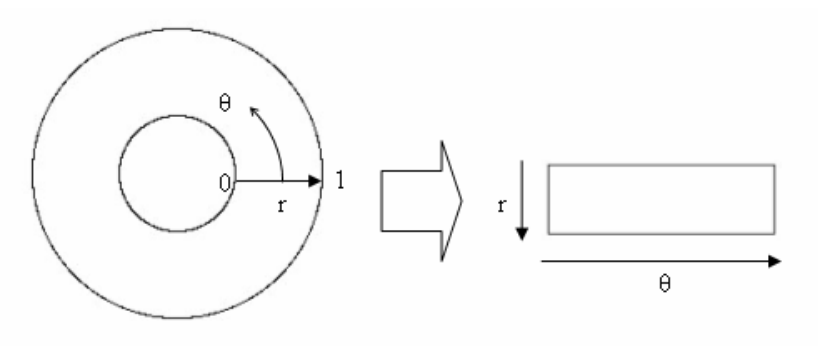
\includegraphics[width=0.8\textwidth]{images/normalization/schemaCenter.png}
  \centering
  \caption{Model normalizacji Daugmana \cite{masek}}
  \label{fig:daugmanDiagram}
\end{figure}

Wybrany rozmiar prostokąta decyduje o ilości informacji znajdujących się w znormalizowanym obrazie.
Wiersze w tak uzyskanym prostokącie można interpretowa\'c jako kolejne okręgi na obrazie tęczówki.
Jak wida\'c na powyższym rysunku \ref{fig:daugmanDiagram}, wybrana wysokoś\'c prostokąta decyduje
o ilości okręgów - rozdzielczoś\'c promieniowa , a szerokoś\'c prostokąta decyduje o rozdzielczości kątowej.\newline

Przejście ze współrzędnych kartezjańskich $(x,y)$ do współrzędnych biegunowych $(r,\theta)$ opisane zostało
przez Daugmana \cite{DaugmanHowIrisRecognitionWorks} równaniami \ref{eq:norm}:

\begin{equation}
  \begin{aligned}
    &I(x(r,\theta), y(r,\theta)) \rightarrow I(r,\theta),
    \\
    \\
    &x(r,\theta) = (1-r)x_{p}(\theta) + rx_{s}(\theta),
    \\
    &y(r,\theta) = (1-r)y_{p}(\theta) + ry_{s}(\theta),
  \end{aligned}
  \label{eq:norm}
\end{equation}

\noindent
gdzie:\\
\indent $x_{p}$, $y_{p}$ - współrzędne na okręgu granicznym \'zrenicy wzdłuż kierunku $\theta$,\\
\indent $x_{s}$, $y_{s}$ - współrzędne na okręgu granicznym tęczówki wzdłuż kierunku $\theta$.\newline

Tak jak wcześniej wspomniano, środki \'zrenicy i tęczówki nie zawsze znajdują się na jednej osi.
Z tego względu wyznaczając kolejne punkty znormalizowanego obrazu należy uwzględni\'c różną odległoś\'c
między granicą \'zrenicy a tęczówki w zależności od rozpatrywanego kąta $\theta$, co dobrze zobrazowane
zostało na rysunku \ref{fig:daugmanDiagramOffCenter}. Niezależnie od tych różnic, wzdłuż każdego kierunku
$\theta$ wybierana jest stała liczba punktów w taki sposób, aby otrzymany obraz był prostokątem
o stałych wymiarach.

\begin{figure}[ht]
  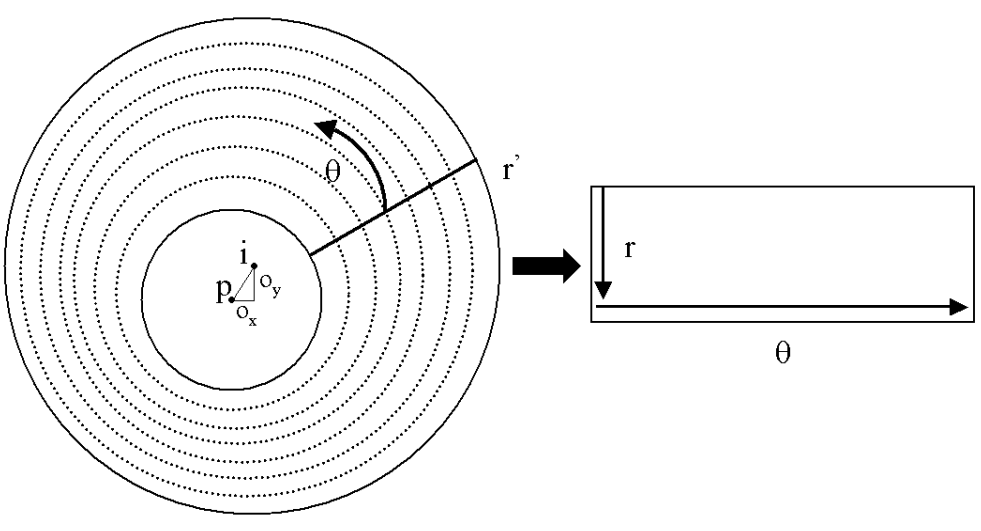
\includegraphics[width=0.8\textwidth]{images/normalization/schemaOffCenter.png}
  \centering
  \caption{Model normalizacji Daugmana z uwzględnieniem niewspółosiowości tęczówki i \'zrenicy \cite{aliasingIris}}
  \label{fig:daugmanDiagramOffCenter}
\end{figure}

Uwzględnienie tej niewspółosiowości polega na wyznaczeniu wartości odległości między granicami
\'zrenicy i tęczówki dla każdego rozpatrywanego kąta \cite{masek} zgodnie z równaniami \ref{eq:normRemap}.

\begin{equation}
  \begin{aligned}
    &r^{\prime} = \sqrt{\alpha}\beta \pm \sqrt{\alpha\beta^{2} - \alpha - r_{I}^{2}},
    \\
    \\
    &\alpha = o_{x}^{2} + o_{y}^{2},
    \\
    &\beta = \cos \left( \pi - \arctan \left( \frac{o_{y}}{o_{x}} \right) - \theta \right).
  \end{aligned}
  \label{eq:normRemap}
\end{equation}

\noindent
gdzie:\\
\indent $o_{x}, o_{y}$ - różnica położeń między środkiem \'zrenicy i tęczówki,\\
\indent $r^{\prime}$ - odległoś\'c między granicą \'zrenicy, a granicą tęczówki pod kątem $\theta$,\\
\indent $r_{I}$ - promień tęczówki\newline

Jeżeli w procesie segmentacji wygenerowana została dodatkowo maska zawierająca informacje o
zakłoceniach znajdujących się w obrębie tęczówki, takich jak powieki, czy rzęsy, wygenerowaną
maskę również należy podda\'c procesowi normalizacji, aby umożliwi\'c korzystanie z niej podczas
porównywania tęczówek. Przykład procesu normalizacji przedstawiony został na rysunku \ref{fig:normalizationExample}.

\begin{figure}[ht]
  \centering
  \begin{subfigure}[b]{0.35\textwidth}
    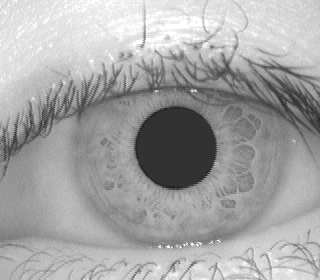
\includegraphics[width=\textwidth]{images/normalization/original.png}
    \caption{Obraz oryginalny}
  \end{subfigure}
  \begin{subfigure}[b]{0.35\textwidth}
    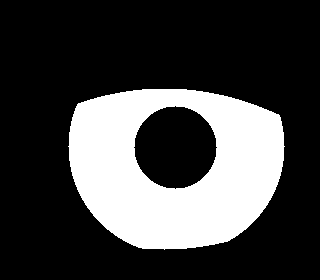
\includegraphics[width=\textwidth]{images/normalization/mask.png}
    \caption{Maska zakłóceń}
  \end{subfigure}
  \begin{subfigure}[b]{0.35\textwidth}
    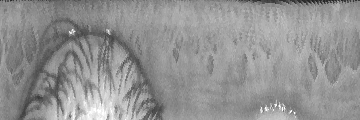
\includegraphics[width=\textwidth]{images/normalization/irisNormalized.png}
    \caption{Tęczówka po normalizacji}
  \end{subfigure}
  \begin{subfigure}[b]{0.35\textwidth}
    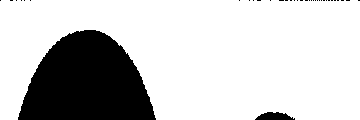
\includegraphics[width=\textwidth]{images/normalization/maskNormalized.png}
    \caption{Maska zakłóceń po normalizacji}
  \end{subfigure}
  \caption{Przykład normalizacji metodą Daugmana}
  \label{fig:normalizationExample}
\end{figure}

Takie rozwiązanie zapewnia odpornoś\'c na rozszerzanie i kurczenie się \'zrenicy, niewspółosiowoś\'c
okręgów tęczówki i \'zrenicy a także różnicę położenia ich między różnymi obrazami. Metoda ta nie
kompensuje jednak różnic rotacji tęczówki. Kompensacja ta jest natomiast zapewniana w procesie
dopasowywania obrazów, który opisany został w pó\'zniejszej części tego rozdziału.

\section{Kodowanie}

Kodowanie tęczówki można rozumie\'c jako opis jej cech.
Dobry algorytm ekstrakcji cech sprawi, że wynik miary dopasowania dla obrazów tej samej tęczówki
będzie znajdował się w innym przedziale niż podczas porównywania obrazów dwóch
różnych tęczówek. Dzięki temu w końcowym etapie procesu rozpoznawania możliwe jest podjęcie decyzji
o rozpoznaniu bąd\'z nierozpoznaniu tęczówki.

Aby zapewni\'c dobrą jakoś\'c identyfikacji tęczówki, proces kodowania powinien wyciąga\'c
z obrazu tylko najważniejsze i najbardziej rozróżnialne jego cechy.
Oppenheim i Lim \cite{OppenheimLim} pokazali w swojej pracy, że najważniejsze
cechy obrazu niesie ze sobą widmo fazowe. Widmo amplitudowe zawiera
informacje o mniej indywidualnych cechach, a także jest zależne od czynników zewnętrznych takich
jak kontrast czy oświetlenie. Z tego względu podczas kodowania tęczówki wykorzystane
powinno by\'c właśnie widmo fazowe obrazu. W celu jego uzyskania należy przenieś\'c znormalizowany
obraz z dziedziny przestrzennej do dziedziny częstotliwości.\newline

Daugman \cite{DaugmanHowIrisRecognitionWorks} w swojej pracy zaproponował użycie w tym celu
filtrów Gabora, dzięki którym można uzyska\'c połączoną reprezentację obrazu w przestrzeni
oraz częstotliwości. Filtry te powstają w wyniku modulacji sinusoidy oraz cosinusoidy za pomocą
funkcji Gaussowskiej.
Częstotliwoś\'c środkowa filtru wyznaczana jest przez częstotliwoś\'c sinusoidy, natomiast
przepustowoś\'c filtru określana jest przez szerokoś\'c wykorzystanej funkcji Gaussowskiej.

Jedną z wad filtrów Gabora jest występowanie niezerowej składowej stałej dla przepustowości
większej niż jedna oktawa \cite{FieldGaborOctave}. Zerową składową stałą dla każdej przepustowości
można natomiast otrzyma\'c przez zastosowanie filtru, którego charakterystyka częstotliwościowa
amplitudowa ma rozkład Gaussowski nie w skali liniowej, a w skali logarytmicznej. Charakterystyka
częstotliwościowa amplitudowa takiego filtru jest opisana równaniem \ref{eq:logGabor}:

\begin{equation}
  \mathit{G(f)} = \exp\left(
  \frac{
    -\left( \log\left( f / f_{0}\right)\right)^{2}
  }{
    2\left(\log\left( \sigma / f_{0}\right)\right)^{2}
  }
  \right),
  \label{eq:logGabor}
\end{equation}

\noindent
gdzie:\\
\indent $f_{0}$ - częstotliwoś\'c środkowa filtra,\\
\indent $\sigma$ - przepustowoś\'c filtra.\newline

W celu zakodowania cech charakterystycznych znormalizowanego obrazu tęczówki, dla każdego wiersza
obrazu obliczany jest jego splot z falkami Log Gabora. Jeżeli moduł wyniku splotu w danym punkcie
jest bardzo blisko zera, wówczas informacja fazowa jest nieznacząca, a punkt ten oznaczany jest w
masce zakłóceń jako bit nieznaczący.

Wynik splotu obrazu z filtrem jest następnie poddawany kwantyzacji \cite{DaugmanHowIrisRecognitionWorks} do czterech wartości odpowiadających
czterem \'cwiartkom płaszczyzny zespolonej przez sprawdzenie znaku częsci rzeczywistej i urojonej
uzyskanego wyniku. Proces kwantyzacji przedstawiony jest na rysunku \ref{fig:encodingQuant}. W wyniku
kwantyzacji znormalizowany obraz tęczówki przekształcany jest do wzoru tęczówki w postaci ciągu bitów.
Przykładowy proces kodowania przedstawiony został na rysunku \ref{fig:gaborEncoding}

\begin{figure}[ht]
  \centering
  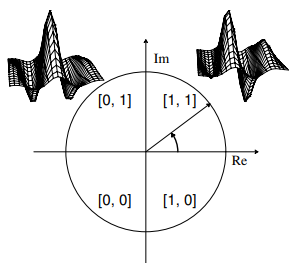
\includegraphics{images/encoding/quantization.png}
  \caption{Ilustracja procesu kwantyzacji}
  \label{fig:encodingQuant}
\end{figure}

W celu uzyskania większej ilości informacji o tęczówce możliwe jest zastosowanie kilku filtrów
Gabora o różnych parametrach. Wówczas obraz poddawany jest splotowi z każdym z takich filtrów, w
związku z czym powielana jest liczba bitów kodujących każdy punkt tęczówki.

Z każdym punktem na obrazie tęczówki związana jest pojedyńcza wartoś\'c w masce zakłóceń. W wyniku
procesu kodowania każdy element obrazu jest reprezentowany przez przynajmniej dwie wartości. W związku
z tym należy zaktualizowa\'c maskę zakłóceń, aby miała ona ten sam rozmiar co otrzymany wzór tęczówki.
W tym celu każdy bit w masce zakłóceń jest powielany tyle razy, ile wartości reprezentuje pojedyńczy
punkt we wzorze tęczówki. Przykładowo, jeżeli w procesie kodowania wykorzystany został jeden filtr,
transformacja przykładowej maski wyglądałaby następująco:

\begin{figure}[ht]
  \centering
  $0|1|1|0|0|1 \rightarrow 00|11|11|00|00|11$
\end{figure}

\begin{figure}[!ht]
  \centering
  \makebox[\textwidth]{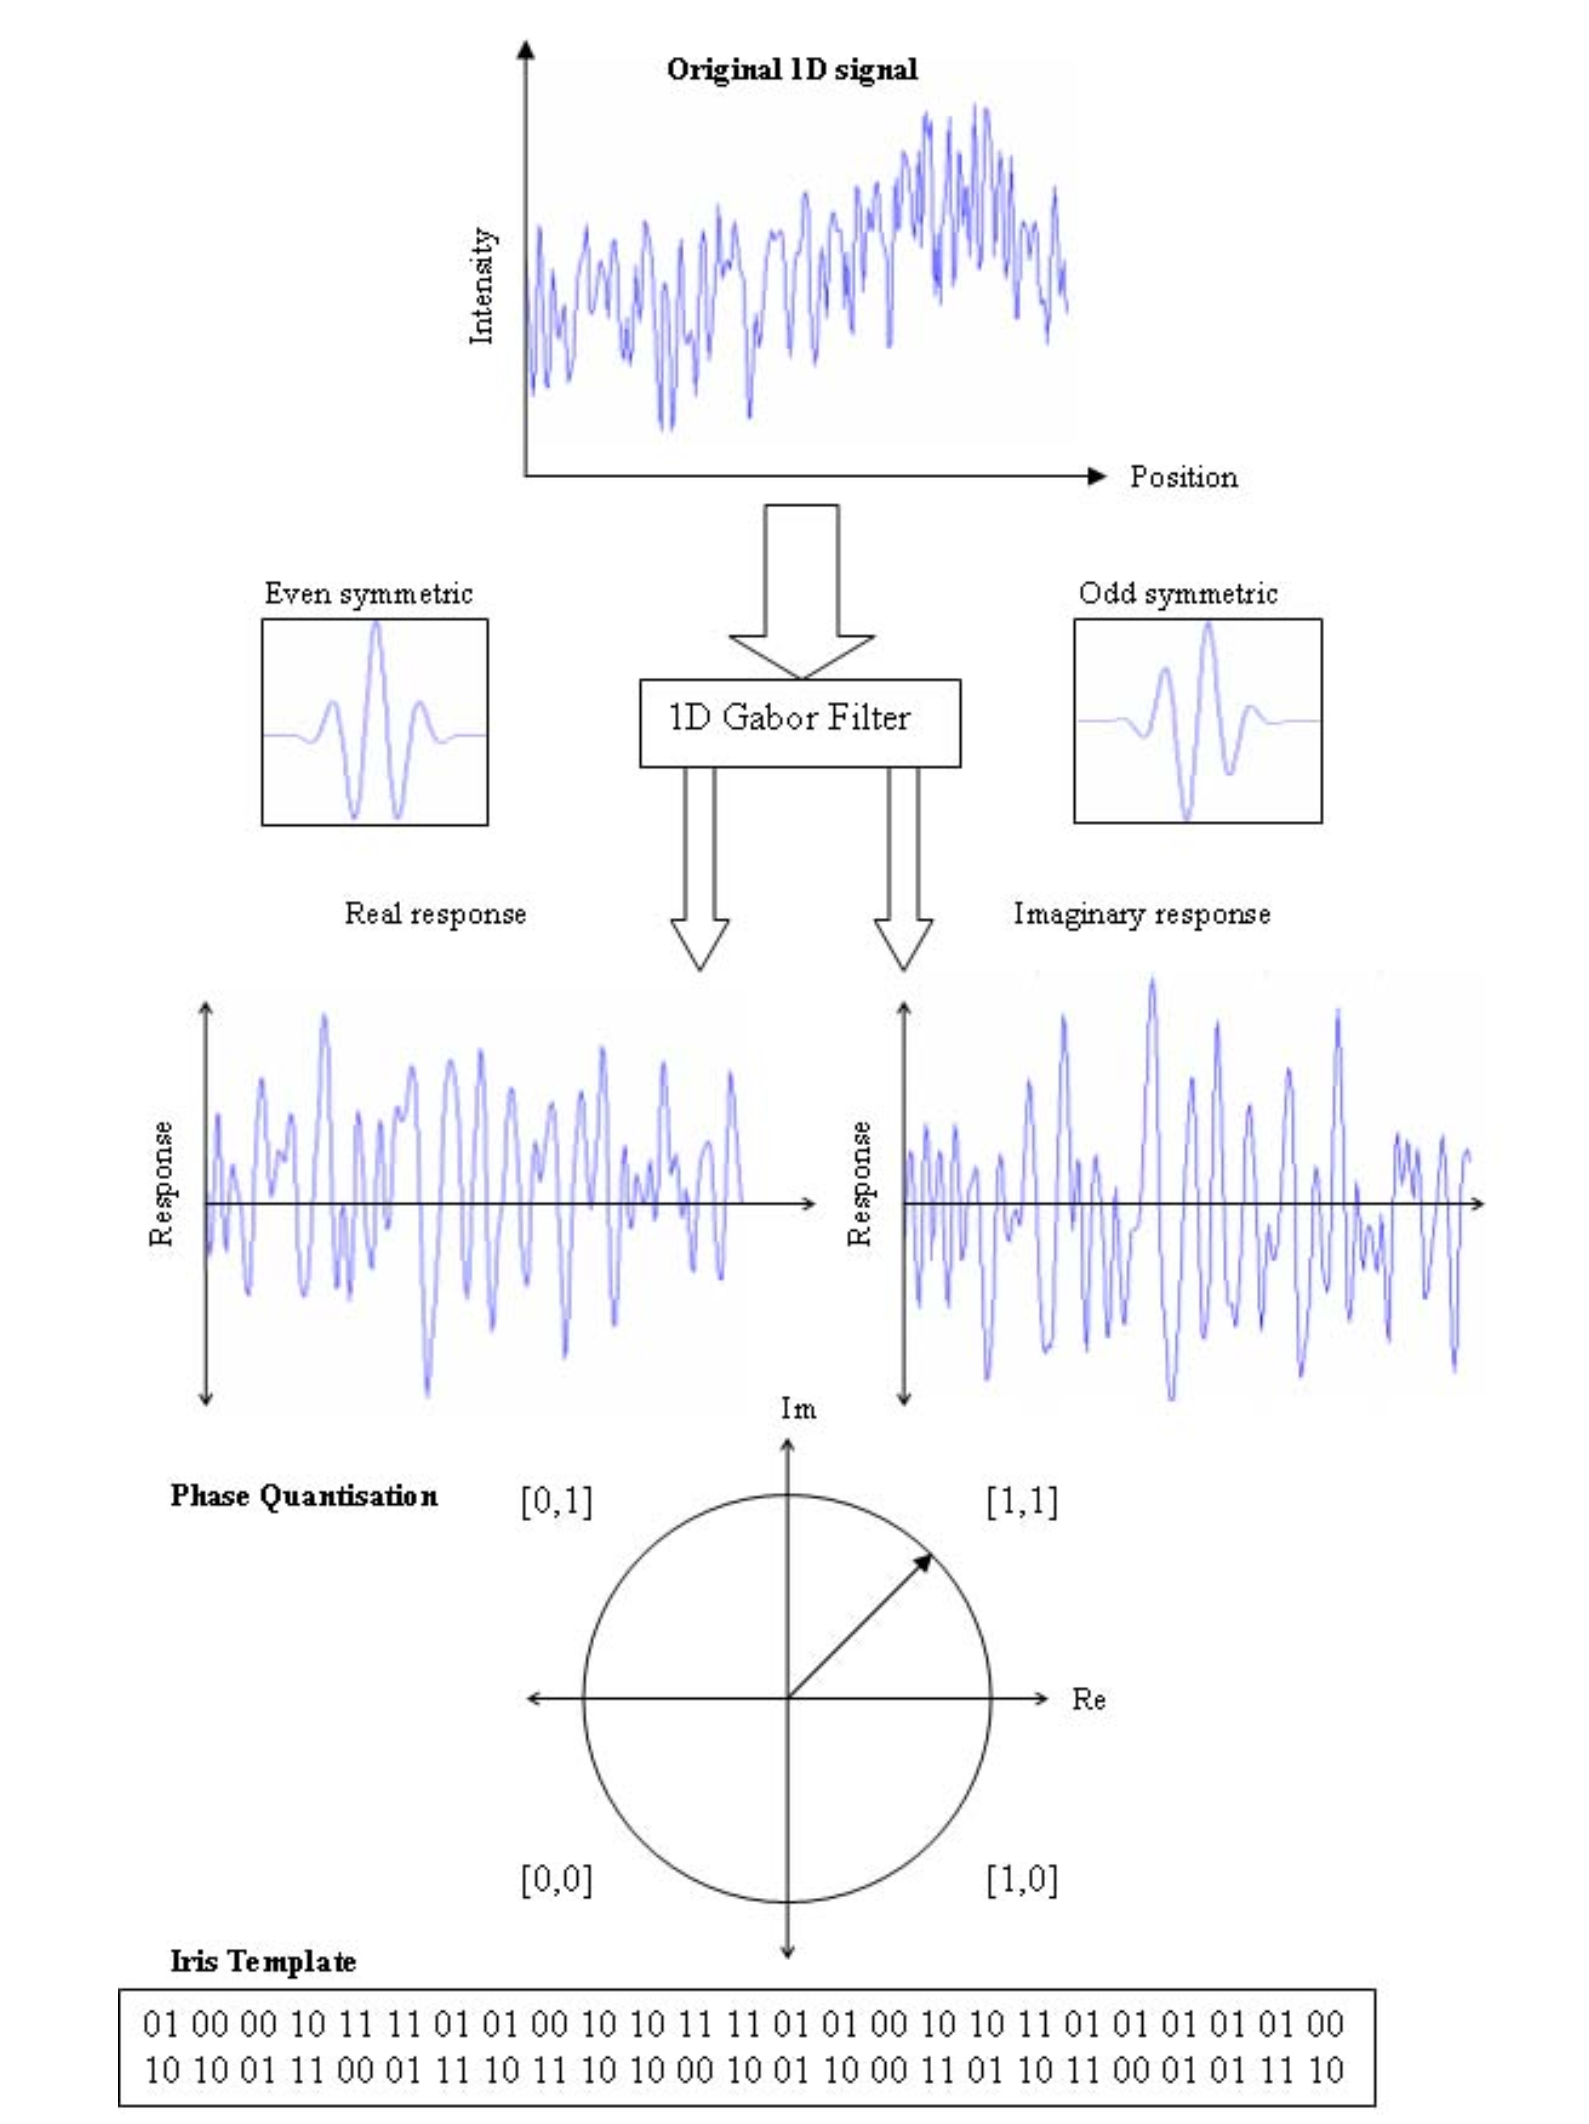
\includegraphics[width=\textwidth,height=\textheight,keepaspectratio]{images/encoding/gabor.png}}
  \caption{Ilustracja procesu kodowania}
  \label{fig:gaborEncoding}
\end{figure}

Na rysunku \ref{fig:gaborExample} przestawiony został przykładowy wynik procesu kodowania zaimplementowanego
w tej pracy.

\begin{figure}
  \centering
  \begin{subfigure}[b]{0.5\textwidth}
    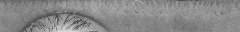
\includegraphics[width=\textwidth]{images/encoding/norm.png}
    \caption{Znormalizowany obraz tęczówki}
  \end{subfigure}
  \begin{subfigure}[b]{0.5\textwidth}
    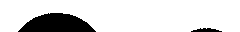
\includegraphics[width=\textwidth]{images/encoding/normMask.png}
    \caption{Znormalizowana maska zakłóceń}
  \end{subfigure}
  \begin{subfigure}[b]{1\textwidth}
    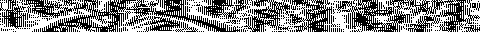
\includegraphics[width=\textwidth]{images/encoding/encoded.png}
    \caption{Wzór tęczówki obrazu znormalizowanego}
  \end{subfigure}
  \begin{subfigure}[b]{\textwidth}
    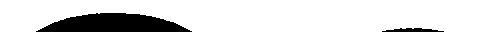
\includegraphics[width=\textwidth]{images/encoding/encodedMask.png}
    \caption{Dostosowana maska zakłóceń do nowego rozmiaru}
  \end{subfigure}
  \caption{Wyniki przykładowego kodowania za pomocą filtrów Gabora.}
  \label{fig:gaborExample}
\end{figure}

\section{Dopasowanie}

W procesie kodowania obraz tęczówki przekształcony zostaje do wzoru tęczówki w postaci ciągu bitowego,
dzięki czemu porównanie dwóch obrazów tęczówek sprowadza się do porównania dwóch ciągów bitowych.
Stopień różnicy między dwoma wzorami tęczówki, można określi\'c obliczając odległoś\'c Hamminga. Mówi
ona o liczbie miejsc, w których dwa słowa bitowe przyjmują różne wartości.
Ustalając pewien próg wartości odległości Hamminga można podją\'c decyzję, czy dwa dane ciągi
reprezentują tę samą tęczówkę.

Wyznaczenie progu dla odległości Hamminga zdefiniowanej w ten sposób zależałoby od długości
porównywanych ciągów bitowych. Aby uniezależni\'c wartoś\'c progu od tej długości, miarę można
zdefiniowa\'c jako sumę niezgodnych bitów podzieloną przez całkowitą liczbę bitów \ref{eq:basicHD}:

\begin{equation}
  \mathit{HD} = \frac{1}{N}\sum\limits_{j=1}^{N}X_{j} \oplus Y_{j},
  \label{eq:basicHD}
\end{equation}

\noindent
gdzie:\\
\indent $X_{j}, Y_{j}$ reprezentują wartości bitów na miejscu $j$ w ciągach odpowiednio $X$ oraz $Y$,\\
\indent $N$ - długoś\'c ciągów $X$ i $Y$,\\
\indent $\oplus$ - operator alternatywy rozłącznej.\newline

W trakcie procesu kodowania oprócz wzoru tęczówki tworzony jest także wzór dla maski zakłóceń.
Zawiera on informacje o tym, które bity we wzorze tęczówki reprezentują tęczówkę i powinny by\'c
uwzględnione, a które bity reprezentują zakłócenia takie jak powieki, czy rzęsy i nie powinny by\'c
porównywane w procesie dopasowywania.\\
Jako że porównywane są dwa obrazy, generowane są również dwie maski zakłóceń i należy uwzględni\'c
każdą z nich. Ponieważ elementy znaczące w masce zakłóceń oznaczone zostały kolorem białym, co odpowiada
wartości $1$ w postaci bitowej. Ostateczną maskę dla procesu dopasowania można zdefiniowa\'c jako
iloczyn logiczny tych dwóch masek - w ten sposób stworzony zostanie jeden ciąg bitowy reprezentujący
bity znaczące za pomocą wartości $1$ oraz bity nieznaczące za pomocą wartości $0$.
Równanie \ref{eq:maskedHD} przedstawia definicję odległości Hamminga z uwzględnieniem obu masek zakłóceń:

\begin{equation}
  \mathit{HD} = \frac{1}{\sum\limits_{j=1}^{N} \left( \mathit{Xm}_{j} \cap \mathit{Ym}_{j} \right) }
       \sum\limits_{k=1}^{N} \left(X_{k} \oplus Y_{k} \right) \cap \left( \mathit{Xm}_{k} \cap \mathit{Ym}_{k} \right),
  \label{eq:maskedHD}
\end{equation}

\noindent
gdzie:\\
\indent $X, Y$ - wzory tęczówki,\\
\indent $\mathit{Xm}, \mathit{Ym}$ - wzory masek zakłóceń dla wzorów tęczówek $X, Y$,\\
\indent $N$ - długoś\'c wzorów tęczówek i masek zakłóceń,\\
\indent $\oplus$ - operator alternatywy rozłącznej,\\
\indent $\cap$ - operator iloczynu logicznego.\newline

Tak jak wcześniej wspomniano, poprzednie procesy w żaden sposób nie uwzględniały możliwości różnic
w rotacji tęczówki na pobranych obrazach. W celu kompensacji tych niespójności podczas procesu
dopasowania jeden z wzorów tęczówki poddawany jest przesunięciom bitowym, które odpowiadają rotacji
tęczówki o kąt zależny od rozdzielczości kątowej wybranej podczas procesu normalizacji. Maska zakłóceń
odpowiadająca temu wzorowi również poddawana jest tym przesunięciom.
Jedno przesunięcie w procesie dopasowania odpowiada dwóm przesunięciom bitowym - jednemu w lewo i
drugiemu w prawo, z których oba wykonywane są względem oryginalnego wzoru tęczówki. Proces ten
zobrazowany został na rysunku \ref{fig:matchingShifting}

\begin{figure}
  \centering
  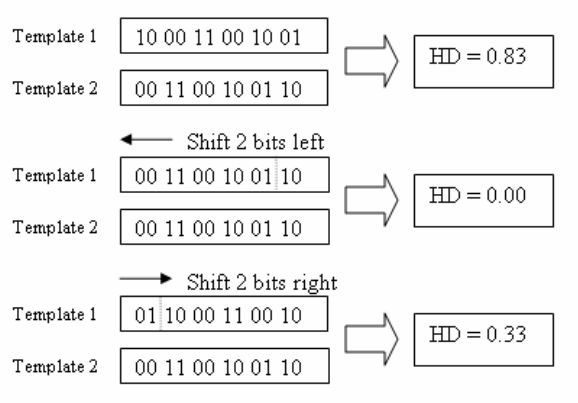
\includegraphics[width=0.6\textwidth]{images/matching/shifting.png}
  \caption{Schemat przedstawiający pojedyńcze przesunięcie wzoru tęczówki. Przykład ten przedstawia
  wzór do wygenerowania którego wykorzystany został jeden filtr Gabora \cite{masek}.}
  \label{fig:matchingShifting}
\end{figure}

W zależności od tego ile bitów koduje pojedyńczy punkt siatkówki, tyle bitów zmienia swoje miejsca
w trakcie pojedyńczego przesunięcia. Liczba przesuniętych bitów zależy od ilości filtrów Gabora
użytych w procesie kodowania, ponieważ każdy z takich filtrów wygeneruje dwa bity reprezentujące
pojedyńczy punkt siatkówki.

Odległos\'c Hamminga obliczana jest dla każdego z tych przesunię\'c. Decyzja o tym, czy dwa wzory
reprezentują tę samą tęczówkę podejmowana jest na podstawie najmniejszej uzyskanej wartości,
która reprezentuje najlepsze dopasowanie dwóch wzorów. Liczba przesunię\'c potrzebna do kompensacji
niespójności rotacji zależy od tego z jaką dokładnością kątową pobierane są zdjęcia tęczówki.
